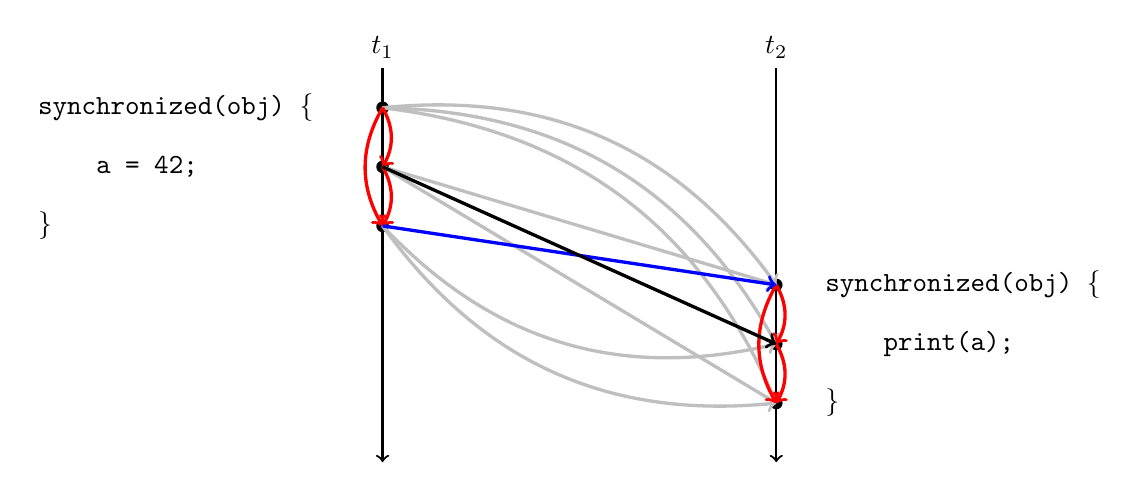
\begin{tikzpicture}
    \draw [->, thick] (4.5,0.5) node[above] {$t_1$} -- (4.5,-4.5);
    \draw (0,0) node[right] {\texttt{synchronized(obj) \{}};
    \coordinate (a1) at (4.5,0);
    \fill (a1) circle (0.08);
    \draw (0,-0.75) node[right] {\texttt{\quad \quad a = 42;}};
    \coordinate (a2) at (4.5,-0.75);
    \fill (a2) circle (0.08);
    \draw (0,-1.5) node[right] {\texttt{\}}};
    \coordinate (a3) at (4.5,-1.5);
    \fill (a3) circle (0.08);

    \draw [->, thick] (9.5,0.5) node[above] {$t_2$} -- (9.5,-4.5);
    \draw (10,-2.25) node[right] {\texttt{synchronized(obj) \{}};
    \coordinate (b1) at (9.5,-2.25);
    \fill (b1) circle (0.08);
    \draw (10,-3) node[right] {\texttt{\quad \quad print(a);}};
    \coordinate (b2) at (9.5,-3);
    \fill (b2) circle (0.08);
    \draw (10,-3.75) node[right] {\texttt{\}}};
    \coordinate (b3) at (9.5,-3.75);
    \fill (b3) circle (0.08);

    \draw[->,color=lightgray,very thick] (a1) to[bend left] (b1);
    \draw[->,color=lightgray,very thick] (a1) to[bend left] (b2);
    \draw[->,color=lightgray,very thick] (a1) to[bend left] (b3);
    \draw[->,color=lightgray,very thick] (a2) to (b1);
    \draw[->,color=lightgray,very thick] (a2) to (b3);
    \draw[->,color=lightgray,very thick] (a3) to[bend right] (b2);
    \draw[->,color=lightgray,very thick] (a3) to[bend right] (b3);

    \draw[->,color=red,very thick] (a1) to[bend left] (a2);
    \draw[->,color=red,very thick] (a2) to[bend left] (a3);
    \draw[->,color=red,very thick] (a1) to[bend right] (a3);

    \draw[->,color=red,very thick] (b1) to[bend left] (b2);
    \draw[->,color=red,very thick] (b2) to[bend left] (b3);
    \draw[->,color=red,very thick] (b1) to[bend right] (b3);

    \draw[->,color=blue,very thick] (a3) to (b1);

    \draw[->,very thick] (a2) to (b2);
\end{tikzpicture}
